%************************************************
\chapter{Search and Navigation in the Presence of Local Cues}\label{ch:hints}
%************************************************
In all previous considerations of search problems we assumed the walker to be completely blind, \ie the search is purely random. However, as we have mentioned before in \autoref{sec:class-search-strategies}, sometimes there are hints in the environment that contain valuable information of the whereabouts of the target. If the searcher is capable of perceiving and analyzing these hints, it can use the additional information in order to adapt its strategy and navigate more efficiently. Some examples include \eg humans reading tracks or dogs sensing odors. However, the perceiving of hints during search is not restricted to more advanced life forms like humans and animals, but can also be observed in simpler organisms like bacteria and cells. In this chapter we will introduce hint-related navigation and search strategies of microorganisms, and we will present related current research.

\section{Directional navigation (Taxis)}
Different organisms are able to detect or sense different types of hints or stimuli in their environment. In the case of \textit{taxis}, the organism is able to gain information about the direction of the stimuli source from the hints in its environment. It then responds to a stimulus with directional movement, \ie it moves towards or away from the source\graffito{Taxis describes guided navigation as a response to a stimulus.}. If the stimulus induces movement towards the source, one speaks of positive taxis, whereas movement away from the source is denoted by negative taxis.

Taxes are generally categorized based on the type of stimulus which induces the response of the organism. A few examples are given in \autoref{tab:taxis-examples}.
\begin{table}[h]
 \myfloatalign
 \begin{tabularx}{\textwidth}{llX} \toprule
  \tableheadline{Term} & \tableheadline{Stimulus} & \tableheadline{Examples of responsive species} \\ \midrule
  Chemotaxis & Chemical & Bacteria, archaea, amoebae, white blood cells, sperm cells \\
  Electrotaxis & Electrical field & Amoebae \\
  Galvanotaxis & Electrical current & Bacteria, spermatozoa \\
  \makecell[tl]{Geotaxis or \\ gravitaxis} & Gravity & Bacteria, ciliates (\textit{Paramecium}), flagellates \\
  Magnetotaxis & Magnetic field & Bacteria \\
  Phototaxis & Light & Bacteria, archaea, amoebae, flagellates \\
  Thermotaxis & Temperature & Bacteria, ciliates, amoebae, nematodes, spermatozoa, trophoblastic cells, leukocytes \\
  \bottomrule
 \end{tabularx}
 \caption[]{Types of taxis with inducing stimuli and examples of responsive species (exert from \cite{eisenbach:2004}).}
 \label{tab:taxis-examples}
\end{table}
In many cases, like \eg chemotaxis and thermotaxis, the response movement occurs up (positive taxis) or down (negative taxis) a gradient.

\subsection{Chemotaxis}
Chemotaxis describes the taxis that is driven by chemical gradients\graffito{Chemotaxis denotes the induced movement along the gradient of the concentration of a chemical.}. Many organisms are attracted or repelled by specific chemicals, as they are beneficial or harmful to them. In case of positive or negative chemotaxis, the inducing chemical is defined as \textit{chemoattractant} or \textit{chemorepellent}, respectively. A food source like \eg glucose is an example for an attractant, whereas a poison like \eg phenol is a repellent. Chemoattractants usually cause accumulation of organisms in locations with high concentrations, whereas chemorepellents lead to depletion in such regions. Note, however, that accumulation and depletion can also be caused by other mechanisms and therefore, they alone cannot be used as an indicator for chemotaxis.

Of course, chemotaxis helps the organism to reduce search times or to more efficiently avoid hazardous chemicals and therefore, in general, it is superior to a purely random movement pattern. Thus, organisms evolve chemotactic responses specific to the environmental conditions which they experience. In steady environments this is feasible, however, in many real environments the conditions fluctuate temporally and spatially. If such fluctuations occur too frequently, the organism is not able to adapt its chemotactic response in time. Therefore, it might be advantageous to omit any chemotaxis and change over to stochastic behavior. An alternative problem is that some environments have different states and a chemotactic response specific to one state might perform poorly in another. When the number of states is low, a specific response can be evolved and molecularly encoded in the organism for each individual state, while for many different states this is not possible. But which response does an organism then evolve in such situations?

This questions was addressed by \mycitea{celani:2010} for the chemotaxis of \textit{Escherichia coli}. \ecoli is known to perform a run-and-tumble like motion comparable to the intermittent search introduced in \autoref{ssec:intermittent-search}. In the presence of chemoattractants the duration of the run phases is modulated. \citeauthor{celani:2010} define the chemotactic response $K(t)$ at time $t$ as the bias in the fraction of time spent in the running vs. the tumbling phase after a pulse of chemoattractant. The switching rate then reads
\begin{equation}
 \omega_{\textrm{run} \rightarrow \textrm{tumble}} = \frac{1}{\tau_\textrm{run}}\left[1-\int\limits^t_{-\infty} K(t-s) c(\bv{X}(s), s) \diff s\right],
\end{equation}
where $\tau_\textrm{run}$ is the mean time spent in the running phase in the absence of any chemoattractant, $c(\bv{x}, t)$ denotes the chemoattractant concentration field, and $\bv{X}(t)$ is the trajectory followed by the bacterium. Thus, $c(\bv{X}(s), s)$ is equivalent to the time history of chemoattractant encounters.

The interesting quantity, in order to compare different chemotactic responses $K(t)$, is the uptake of chemoattractant defined as
\begin{equation}
 S = \int c(\bv{x}, t) n(\bv{x}, t) \diff \bv{x} \diff t,
\end{equation}
where $n(\bv{x}, t)$ is the probability density of the bacterium space-time coordinates, which depends on $K(t)$ in non-trivial ways (see \cite{celani:2010} for further details). Note, that the term uptake does not necessarily mean that the chemical is metabolized, it is rather a quantity that measures the amount of chemical that is encountered by the bacterium along its trajectory. As we consider chemoattractants here, maximizing $S$ by evolving a good response $K(t)$ is beneficial to the bacterium. Now instead of finding the best choice of $K(t)$ in dependence on the chemoattractant profile $c(\bv{x}, t)$, \ie a specific profile, which would be the analog to the evolution of a specific response in steady environments, \citeauthor{celani:2010} consider all possible chemoattractant profiles for a given $K(t)$. The goal of this strategy is to find the chemoattractant profile for which the given $K(t)$ performs the worst, \ie has the minimum uptake, and iterate this step for all $K(t)$s of interest. Then, among all the responses $K(t)$, select the one with the largest minimum uptake. \citeauthor{celani:2010} call this response the \textit{maximin} strategy, as it maximizes the uptake among all the worst-case responses.

The chemotactic responses $K(t)$ that are considered are of the form
\begin{equation}
 K(t) = \lambda e^{-\lambda t} \left[\beta_1 \lambda t + \beta_2 (\lambda t)^2\right],
\end{equation}
where $\lambda$ controls the rescaling of the time variable, and $\beta_1, \beta_2$ specify the amplitude and the shape of $K(t)$. Furthermore, the parameter $\gamma$ is introduced as
\begin{equation}
 \gamma \propto \int\limits_0^\infty K(t) \diff t,
\end{equation}
in order to represent the bacterial response with a single variable.

The chemoattractant profiles $c(\bv{x},t)$ that are considered are of parabolic form with a rapid exponential decay in time, \ie
\begin{equation}
 c(\bv{x},t) \propto e^{-t / \tau_c},
\end{equation}
where $\tau_c$ is the degradation time. In the supporting material of \cite{celani:2010} one can find explanations to why such profiles are sufficient. Because of the rapid decay in time, it is furthermore sufficient to only consider the local properties of the chemoattractant profile around the bacterial position. These local properties are also expressed by a single variable.

From the different bacterial responses and chemoattractant profiles \citeauthor{celani:2010} then derive a phase space for the uptake, which is shown in \autoref{fig:uptake-phase-space}.

\begin{figure}[bth]
 \myfloatalign
 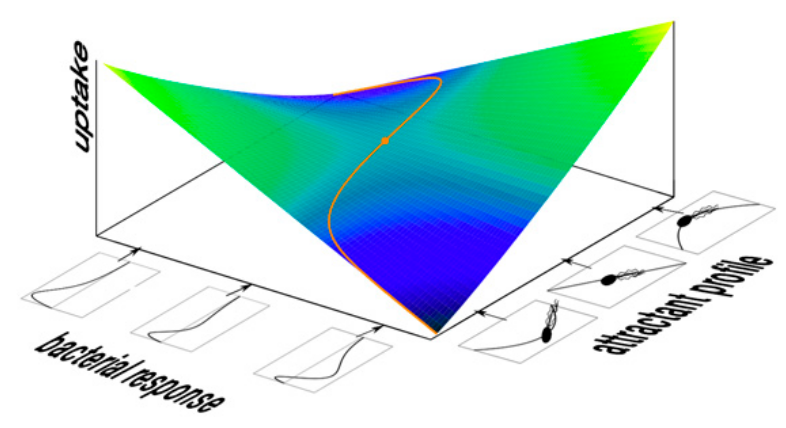
\includegraphics[width=0.8\linewidth]{gfx/uptake-phase-space}
 \caption[]{A schematic view for the phase space of the chemoattractant bacterial uptake $S$. The bacterial responses are represented by the parameter $\gamma$. Three exemplary response functions $K(t)$ with positive, zero, and negative $\gamma$ are shown. Chemoattractant profiles $c(\bv{x},t)$ are also represented by a single variable that condenses information about the local profile around the bacterial position. Responses with negative $\gamma$ are advantageous in keeping the bacterium localized around a maximum of chemoattractant concentration and disadvantageous in escaping from a minimum. The opposite holds true for positive values of $\gamma$. Thus, extreme values of $\gamma$ perform well under particular conditions and bad under others. The minimum uptake of chemoattractant for each bacterial response is indicated by the orange line; the orange circle marks the maximum among these minima (maximin strategy) \cite{celani:2010}.}\label{fig:uptake-phase-space}
\end{figure}

What they find is that a chemotactic response $K(t)$ having a zero integral $\gamma = 0$ guarantees the highest minimal uptake of chemoattractants (maximin strategy), irrespectively of the chemoattractant profile. Furthermore, experimental data on the chemotactic response $K(t)$ of \ecoli to aspartate is in good agreement with the theoretical prediction for $K(t)$ as shown in \autoref{fig:experimental-bacterial-response}.

\begin{figure}[bth]
 \myfloatalign
 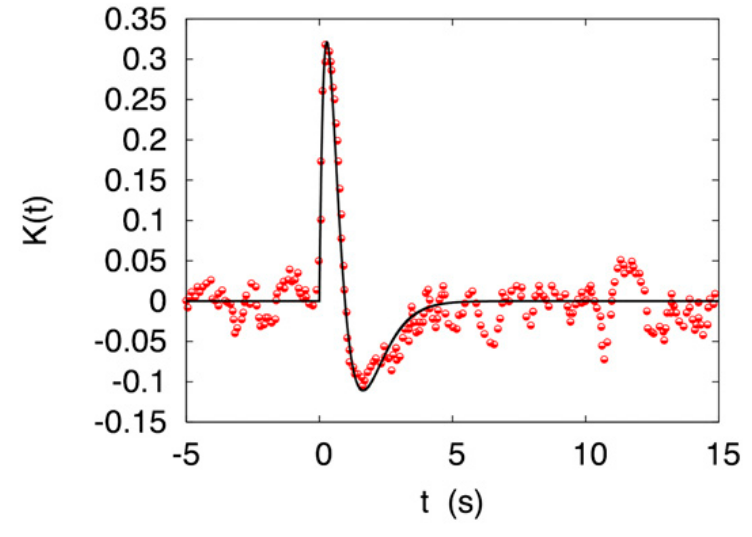
\includegraphics[width=0.8\linewidth]{gfx/experimental-bacterial-response}
 \caption[]{The experimental chemotactic response $K(t)$ of \ecoli to aspartate (red circles). Bacteria are subject to a pulse of chemoattractant at $t=0$. The positive and negative lobes of the response have approximately equal area, which corresponds to $\gamma = 0$. The solid black line is the theoretical prediction of the maximin strategy \cite{celani:2010}.}\label{fig:experimental-bacterial-response}
\end{figure}

But how can these results be explained? First of all, the zero integral filters out low-frequency (namely, constant) parts of $c(\bv{x},t)$ and thus enables an efficient sensing of its gradient, independent of the background level. Additionally, we can understand the impact of the parameter $\gamma$ if we consider its influence on the bacterial movement. Navigation with $\gamma < 0$ reduces the effective diffusivity, which is bad for escaping minima in the concentration profile, whereas positive $\gamma >0 $ increases diffusivity, which again is bad for staying around maxima. However, $\gamma \neq 0$ is not a bad chemotactic response per se as they outperform $\gamma = 0$ responses for specific chemoattractant profiles, \ie we have a classical specialist vs. generalist trade-off situation, in which the generalist wins when performance is compared considering \emph{all} chemoattractant profiles. Indeed, \citeauthor{celani:2010} find that the maximin response is the only one that outperforms motile nonchemotactic bacteria, \ie $K(t) \equiv 0$, in all chemoattractant profiles.

This example shows that the choice of a chemotactic strategy heavily depends on the environmental conditions and justifies the use of chemotaxis as compared to random diffusion even in the case of rapidly changing environments. Nevertheless, changing environments among other factors can still be a reason to use a different strategy which will be introduced below.


\section{Non-directional navigation (Kinesis)}
Similar to the case of taxis, in \textit{kinesis} organisms are able to react to certain stimuli in the environment. However, the organism does not gain information about the direction of the stimuli source and thus is not able to respond with directed movement.\graffito{Kinesis describes a change in activity as a response to a stimulus.} Instead, the organism responds with a change in activity, such as a change in \eg velocity or persistency, which is dependent upon the stimulus intensity. As stimuli do not induce directed movement, there is no positive or negative kinesis as in the case of taxis.

Similarly to taxes, kinesis responses are also categorized based on the type of stimulus which induces the change of activity (see \autoref{tab:taxis-examples}). In some organisms, such as sperm cells, taxis and kinesis may even occur in parallel.

\subsection{Chemokinesis}
Chemokinesis, similarly to chemotaxis, describes the kinesis which is driven by chemical concentrations. Rather than measuring gradients, here the organisms are only able to measure an absolute concentration. As most sources secrete chemicals in spherical symmetry, the concentration is directly connected to the distance to the source and thus, the organism is able to estimate how far away the source is located.

Chemokinesis is not as well researched and understood as its taxis counterpart and one might wonder why chemokinesis even exists, considering that chemotaxis is a superior strategy in finding the target. There are several confounding factors which limit the effectiveness of chemotaxis. As we have seen above, gradients can fluctuate strongly in natural environments and even though in such cases a chemotactic strategy still outperforms random diffusion, possibly a chemokinesis strategy performs even better. Furthermore, instead of fluctuating gradients one could have totally chaotic fields or very weak gradients, which appear constant to the sensing tools of the organism. Sometimes information is only sparse and therefore no gradient is available at all. In all of these scenarios the determination of the direction would fail, rendering chemotaxis useless. The chemotactic navigation is further influenced by external, internal and ligand-receptor binding noise \cite{patnaik:2012}. Delayed responses, as schematically shown in \autoref{fig:chemotacticResponse}, can also lead to wrong navigation.

\begin{figure}[bth]
    \myfloatalign
    \subfloat[][]{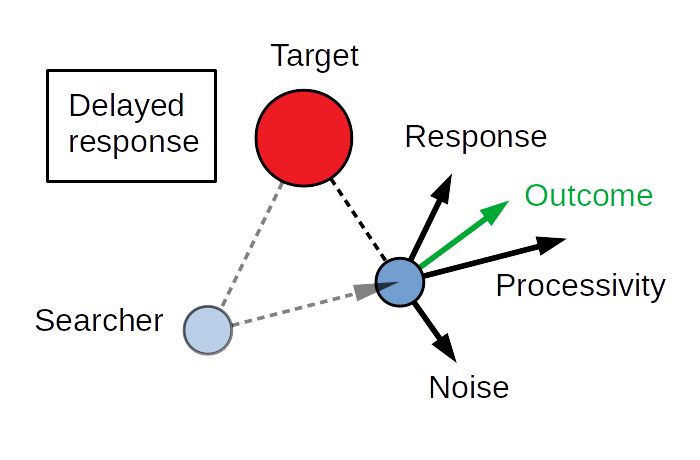
\includegraphics[width=.45\linewidth]{gfx/delayedResponse2}} \quad
    \subfloat[][]{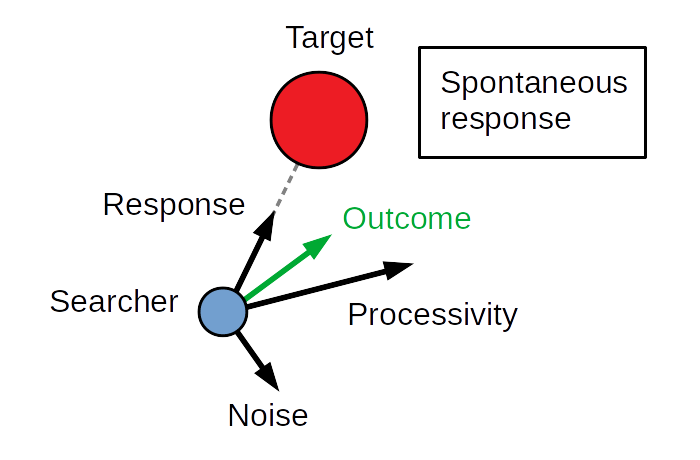
\includegraphics[width=.45\linewidth]{gfx/spontaneousResponse2}}
    \caption[]{Schematic comparison of a delayed response (a) and a spontaneous response (b) in chemotactic navigation in the presence of other sources of error. Here, the delayed response leads to an inefficient navigation, \ie the distance to the target may be even increased.}\label{fig:chemotacticResponse}
\end{figure}

And last but not least, the sensing of gradients as compared to concentrations requires more advanced molecular abilities or memory, and therefore, it is not available to very simple organisms.

\subsection{Durokinesis}
Another example of kinesis is \textit{durokinesis}, which describes rigidity driven kinesis. This means that the organism changes its activity according to the stiffness of the substrate it is moving on.

Most cells, for example, feature migration up a rigidity gradient \cite{novikova:2017}. This feature had been referred to as durotaxis, as the migration happens along a gradient and therefore seems to be comparable to chemotaxis. As we have outlined earlier, chemotaxis obviously is beneficial to organisms, however the advantage of durotaxis is questionable or at least less obvious. Therefore, \mycitea{novikova:2017} took a closer look at this phenomenon in order to figure out whether it is a matter of taxis or not. Additionally, it was observed that the persistency of cellular motion itself changes with the rigidity of the substrate. Especially this observation gave rise to the question whether the overall motion along the gradient can be the consequence of a locally changing persistency alone. In this case, cells would not gain any directional information from the gradient, such as in taxis navigation, but they would only change their activity, \ie their persistency, according to local information. Nonetheless, this would mean that the outcome of durokinesis and taxis strategies is similar, namely migration in response to a gradient.

In their simulation setup, \citeauthor{novikova:2017} consider two-dimensional substrates with different constant and linear rigidity profiles along one dimension (x-axis). The rigidity is directly connected to the persistency, which is controlled by the persistence time $\tau_p$, a quantity occurring in the \ac{msd} of a \ac{prw}
\begin{equation*}
 \avg{|\bv{x}^2|}(t) = 2 v_c^2 \tau_p^2 \left(\frac{t}{\tau_p} + e^{-t/\tau_p} - 1\right),
\end{equation*}
where $v_c$ denotes the cell migration speed \cite{novikova:2017}. \autoref{fig:constantRigidity} shows the influence of soft and stiff substrates and hence different persistence on cell migration. As one can see, the covered area is much larger in the case of higher persistency.

\begin{figure}[bth]
    \myfloatalign
    \subfloat[][]{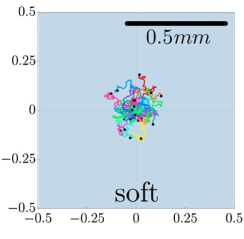
\includegraphics[width=.4\linewidth]{gfx/soft}} \quad
    \subfloat[][]{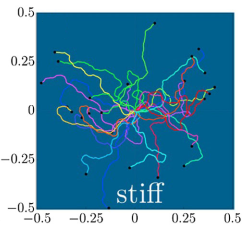
\includegraphics[width=.4\linewidth]{gfx/stiff}}
    \caption[]{Simulated cell migration at different values of persistency, for constant low persistence time $\tau_p = \SI{0.2}{\hour}$ (a) and constant high persistence  time \mbox{$\tau_p = \SI{2}{\hour}$ (b).} In both cases 25 cell trajectories have been recorded over a total time of \SI{12}{\hour}. Trajectories start at the origin and end at the black dots \cite{novikova:2017}.}\label{fig:constantRigidity}
\end{figure}

However, the effect of rigidity gradients is more interesting. Therefore, they introduce a gradient region that occupies a part of the substrate and is flanked by uniformly rigid regions. Within the gradient region, the persistence time increases linearly from \SI{0.2}{\hour} to \SI{12}{\hour} over the whole range and remains constant outside. By changing the width of the gradient region they realize different gradient steepnesses. The result for one of these realizations is shown in \autoref{fig:gradientRigidityA}. One can see that migration happens preferentially in the direction of increasing stiffness, just as it would be the case in durotaxis, however, by the simulation setup, the cells do not sense the gradient at all, they only change their persistency according to local information, \ie the local stiffness. Furthermore, with increasing steepness of the gradient, the average displacement in gradient direction increases as well (\autoref{fig:gradientRigidityB}). Therefore, the rigidity-dependent persistency can indeed explain the migration along the gradient.

\begin{figure}[bth]
    \myfloatalign
    \subfloat[][]{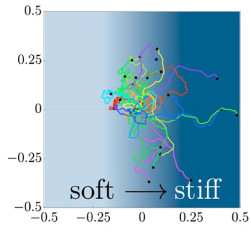
\includegraphics[width=.4\linewidth]{gfx/softToStiff}\label{fig:gradientRigidityA}} \quad
    \subfloat[][]{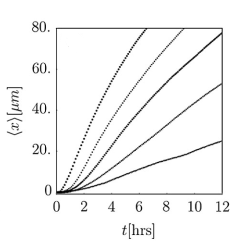
\includegraphics[width=.4\linewidth]{gfx/x-displacement}\label{fig:gradientRigidityB}}
    \caption[]{(a) Simulated cell migration for persistence time $\tau_p$ linearly increasing from \SI{0.2}{\hour} to \SI{12}{\hour} over the x-range $[-0.1, 0.1] mm$ and (b) averaged $x$ displacement for different gradient steepnesses (top to bottom: $\Delta\tau_p / \Delta x = \SI{90}{\hour \per \milli\meter}, \SI{18}{\hour \per \milli\meter}, \SI{9}{\hour \per \milli\meter}, \SI{4.5}{\hour \per \milli\meter}, \SI{1.8}{\hour \per \milli\meter}$) \cite{novikova:2017}.}\label{fig:gradientRigidity}
\end{figure}

Nevertheless, both a purely durokinetic and a durotactic navigation feature migration along a rigidity gradient. So how can one distinguish between both? \citeauthor{novikova:2017} propose to consider the durotactic (vector) index, which is defined as
\begin{equation*}
 \bv{DI}(t) = \left(\begin{array}{c} DI_x(t) \\ DI_y(t) \end{array}\right) \equiv \dfrac{\avg{\bv{x}}(t)}{v_c t},
\end{equation*}
where $\avg{\bv{x}}(t)$ is the average cell displacement. Here, $DI_y(t) = 0$ as there is no bias or gradient in the y-direction and it is sufficient to consider $DI_x(t)$, exclusively. They find, that the durotactic index $DI_x(t)$ of the durokinetic random walk introduced here shows significantly different behavior compared to the durotactic index of a chemotaxis walk with run-and-tumble behavior. While the durotactic index only gradually increases to its plateau value $v_d / v_c$ ($v_d$ being the average velocity in gradient direction) for the durokinetic walk, it rapidly increases for the run-and-tumble walk. Thus, the analysis of the short-time behavior of the durotactic index provides an adequate way to discriminate between the navigation discussed above and a ``regular'' taxis.

\section{Outlook and further directions}

In this last example, the work of \mycitea{novikova:2017}, the properties of a navigation purely based on a kinesis strategy resemble the migrational properties of navigation based on taxis strategies. Therefore, it seems promising to take a look at first-passage time properties of kinesis strategies as well.

In our work, we plan to study active motions with position-dependent activity, where the magnitude of the activity varies as a function of the distance to the target. The ultimate goal is to find the best functionality which optimizes the search time of such a random walker. Among other key parameters, the influence of particle velocity, boundary conditions, and target and system sizes on the search efficiency will be also adressed.


%*****************************************
%*****************************************
%*****************************************
%*****************************************
%*****************************************
